\section{平面电磁波}
    \subsection{电磁场波动方程的导出}
        考虑在没有自由电荷分布的自由空间或均匀绝缘介质中的电磁场运动形式的情况下(即$\rho=0,J=0$的情况下),麦克斯韦方程可以写作
        \begin{equation}
            \label{eq.4_1}
            \begin{gathered}
            \nabla \times \boldsymbol{E}=-\frac{\partial \mathbf{B}}{\partial t} \\
            \nabla \times \mathbf{H}=\frac{\partial \mathbf{D}}{\partial t} \\
            \nabla \cdot \boldsymbol{D}=\rho \\
            \nabla \cdot \mathbf{B}=0
            \end{gathered}
        \end{equation}

        先讨论在真空情形中$\boldsymbol{D}=\varepsilon_{0} \boldsymbol{E}, \boldsymbol{B}=\mu_{0} \mathbf{H}$的情况,联立上述两式,并结合式\ref{eq.4_1}可以得到
            \begin{equation}
                \label{eq.4_2}
                \mu_0 \frac{\partial \boldsymbol{H}}{\partial t} = \frac{\partial \boldsymbol{B}}{\partial t} = - \nabla \times \boldsymbol{E}
            \end{equation}
        上式两边同时取旋度得到
            \begin{equation}
                \nabla \times (\mu_0 \frac{\partial \boldsymbol{H}}{\partial t}) = \mu_0 \frac{ \partial }{\partial t}(\nabla \times \boldsymbol{H}) = \nabla \times (\nabla \times \boldsymbol{E})
            \end{equation}
            \begin{equation}
                -\mu_0 \varepsilon_0 \frac{\partial^2 \boldsymbol{E}}{\partial^2 t} = \nabla \times (\nabla \times \boldsymbol{E}) = \nabla(\nabla \cdot \boldsymbol{E})-\nabla^2 \boldsymbol{E}
            \end{equation}
        根据式\ref{eq.4_1}第三项和第四项可以得到$\nabla \cdot \boldsymbol{E}=0$,整理上式得
            \begin{equation}
                \label{eq.4_5}
                \nabla^2 \boldsymbol{E} - \mu_0 \varepsilon_0 \frac{\partial^2 \boldsymbol{E}}{\partial^2 t} = \nabla^2 \boldsymbol{E} - \frac{1}{c^2} \frac{\partial^2 \boldsymbol{E}}{\partial^2 t}= 0
            \end{equation}
        同理,如果对磁场进行相应的操作可以得到
        \begin{equation}
            \label{eq.4_6}
            \nabla^2 \boldsymbol{H} - \frac{1}{c^2} \frac{\partial^2 \boldsymbol{H}}{\partial^2 t}= 0
        \end{equation}

        式\ref{eq.4_5}和\ref{eq.4_6}统称为波动方程,c是电磁波在真空中的传播速度。请务必明确上面是在没有自由电荷分布的自由空间或均匀绝缘介质中才成立。\footnote{对于介质中的传播形式,我们在这里不赘述,详细请翻阅教材}
    \subsection{时谐电磁波}
        时谐电磁波,即电磁波的激发源以一定频率正弦振荡激发的电磁波称为时谐电磁波,亦称为单色波。一个非时谐的电磁波也可以使用傅立叶分析转化为时谐电磁波的叠加。

        我们讨论一定频率的电磁波,设角频率为$\omega$,电磁场对时间的依赖关系就是$\cos \omega t$,或者以复数的形式代为表示以简化之后的计算量\footnote{我们可以发现转换为复数形式之后其实相较于原来的物理意义多出了$i \sin \omega t$项,国内的大多数教材对于这里的解释是不够清晰的。其实两者在物理意义上是不相等的。这里主要强调的是一种对应关系,以复数形式代为进行计算以简化计算的难度,对应关系和相等关系是有区别的,更为严谨的写法应该是$\boldsymbol{E}(\boldsymbol{x}, t)=\boldsymbol{Re}[\boldsymbol{E}(\boldsymbol{x}) \mathrm{e}^{-\mathrm{i} \omega t}]$。在之后涉及到瞬时能流密度计算的时候会变回实部,我们在那时给出相应的理解。   }
        \begin{equation}
            \begin{aligned}
            &\boldsymbol{E}(\boldsymbol{x}, t)=\boldsymbol{E}(\boldsymbol{x}) \mathrm{e}^{-\mathrm{i} \omega t} \\
            &\boldsymbol{B}(\boldsymbol{x}, t)=\boldsymbol{B}(\boldsymbol{x}) \mathrm{e}^{-\mathrm{i} \omega t}
            \end{aligned}
        \end{equation}
        \begin{equation}
            \begin{gathered}
                e^{-i \omega t}  \\
                cos(\omega t)
            \end{gathered}
        \end{equation}

        代入麦克斯韦方程组可以直接消去共同因子$e^{i \omega t}$得到\footnote{在$\omega \neq 0$的情况下,这四个方程不是独立的,有第一式可以推导第二式,第三式可以推导第四式}
        \begin{equation}
            \begin{gathered}
            \boldsymbol{\nabla} \times \boldsymbol{E}=\mathrm{i} \omega \mu \boldsymbol{H} \\
            \boldsymbol{\nabla} \times \boldsymbol{H}=-\mathrm{i} \omega \varepsilon \boldsymbol{E} \\
            \boldsymbol{\nabla} \cdot \boldsymbol{E}=0 \\
            \boldsymbol{\nabla} \cdot \mathbf{H}=0
            \end{gathered}
            \end{equation}
        
        上一节推导真空电磁场波动方程的流程依然适用,
        \begin{equation}
            \boxed{\nabla \times (\nabla \times \boldsymbol{E}) = \nabla(\nabla \cdot \boldsymbol{E})-\nabla^2 \boldsymbol{E}=-\nabla^2 \boldsymbol{E} = \omega^2 \mu \varepsilon \boldsymbol{E}}
        \end{equation}
        
        得到\footnote{\label{ft.4_1_3}在假定了条件$\nabla \cdot \boldsymbol{E}=0$之后才能够直接写成这种形式},该式称为Helmholtz方程,是一定频率电磁波的基本方程,其解$\boldsymbol{E}(x)$是电磁波场强在空间中的分布情况,每一种可能的形式称为一种波模。
        \begin{equation}
            \begin{gathered}
            \nabla^{2} \boldsymbol{E}+k^{2} \boldsymbol{E}=0 \\
            k=\omega \sqrt{\mu \varepsilon}
            \end{gathered}
            \end{equation} 
        代入麦氏方程可以得到磁场\footnote{如果用磁场的方式给出这个方程,则为\[\begin{aligned}
            \nabla^{2} \boldsymbol{B}+k^{2} \boldsymbol{B} &=0 \\
            \nabla \cdot \boldsymbol{B} &=0 \\
            \boldsymbol{E}=\frac{\mathrm{i}}{\omega \mu \varepsilon} \nabla \times \boldsymbol{B} &=\frac{\mathrm{i}}{k \sqrt{\mu \varepsilon}} \nabla \times \boldsymbol{B}
            \end{aligned}\]
            为保证文本的连贯性,不在正文中直接给出}
        \begin{equation}
            \label{eq.4.11}
            \boldsymbol{B}=-\frac{\mathrm{i}}{\omega} \nabla \times \boldsymbol{E}=-\frac{\mathrm{i}}{k} \sqrt{\mu \varepsilon} \nabla \times \boldsymbol{E}
        \end{equation}
    \subsection{平面电磁波}      
        我们假设一种最基本的解,它是平面波。设电磁波沿x轴方向传播,其场强在与x轴正交的平面上各点具有相同的值。这种情况下Helmholtz方程退化为
        \begin{equation}
            \frac{\mathrm{d}^{2}}{\mathrm{~d} x^{2}} \boldsymbol{E}(\boldsymbol{x})+k^{2} \boldsymbol{E}(\boldsymbol{x})=0
        \end{equation}
        求解上式并加上时谐项可以得到
        \begin{equation}
            \boldsymbol{E}(\boldsymbol{x}, t)=\boldsymbol{E}_{0} \mathrm{e}^{\mathrm{i}(k x-\omega t)} = \boldsymbol{E}(\cos(kx-\omega t)+i \sin(kx-\omega t))
        \end{equation}

        对于实际存在的场强应该理解为上式只取实数部分
        \begin{equation}
            \label{eq.4_14}
            \boldsymbol{E}(\boldsymbol{x}, t)= \boldsymbol{E} \cos(kx-\omega t)
        \end{equation}

        我们直接考虑相位因子$\cos (kx - \omega t)$的意义,它给出了电磁场随位置和时间变化的关系;考虑t=0的情况时,有波峰在x=0处,在$t=1/\omega$时,这一波峰移到$x=1/k$,我们可以计算得到相速度
        \begin{equation}
            \label{eq.4_16}
            v=\frac{\omega}{k}=\frac{1}{\sqrt{\mu \varepsilon}}
        \end{equation}    

        我们已经知道在真空中这一速度是光速,相应的在介质中就可以表示为
        \begin{equation}
            v=\frac{c}{\mu_r \varepsilon_r}
        \end{equation}

        上述的计算是由于我们选择了情况最简单的一个坐标系——波矢量刚好和x轴的方向平行,对于一般的情况波矢量和空间上任意一个位矢应该表示为$\boldsymbol{k} \cdot \boldsymbol{x}$,或者用位矢在波矢量方向上的投影x',记作$k x'$\footnote{这里的k已经退化成一个标量,我们一般称为波数,等于\[k= \frac{2 \pi}{\lambda}\]}。如果我们以x’作垂直于波矢量的平面,就可以得到一个等相位的平面。
        
        在求解式\ref{eq.4_14}之前,我们要明确该式的得出需要满足\ref{ft.4_1_3},我们直接对式\ref{eq.4_14}取散度得到
        \begin{equation}
            \boldsymbol{\nabla} \cdot \boldsymbol{E}=\boldsymbol{E}_{0} \cdot \boldsymbol{\nabla} \mathrm{e}^{\mathrm{i}(\boldsymbol{k} \cdot \boldsymbol{x}-\omega t)}=\mathrm{i} \boldsymbol{k} \cdot \boldsymbol{E}_{0} \mathrm{e}^{\mathrm{i}(\boldsymbol{k} \cdot \boldsymbol{x}-\omega t)}=\mathrm{i} \boldsymbol{k} \cdot \boldsymbol{E}=0
        \end{equation} 
        即
        \begin{equation}
            \boldsymbol{k} \cdot \boldsymbol{E} = 0
        \end{equation}

        表示电场的波动是横波,$\boldsymbol{E}$的取向称为电磁波的偏振方向。如果我们选垂直于$\boldsymbol{k}$的两个相互正交的方向作为偏振方向,我们可以称对于每一个$\boldsymbol{k}$都有两个独立的偏振波。

        下面考虑磁场,根据式\ref{eq.4.11}
        \begin{equation}
            \label{eq.4_20}
            \boldsymbol{B} = -\frac{\mathrm{i}}{k} \sqrt{\mu \varepsilon} [\nabla \mathrm{e}^{\mathrm{i}(\boldsymbol{k} \cdot \boldsymbol{x}-\omega t)}] \times \boldsymbol{E} = \sqrt{\mu \varepsilon}\boldsymbol{e}_k \times \boldsymbol{E}
        \end{equation}
        可以看出同样是横波。且和相位项无关,电场波和磁场波同相。
        \begin{equation}
            \label{eq.4_21}
            \left|\frac{\boldsymbol{E}}{\boldsymbol{B}}\right|=\frac{1}{\sqrt{\mu \varepsilon}}=v
        \end{equation}
        v为当前介质下的光速。
    \subsection{电磁场的能量和能流}      
        由式\ref{eq.1_74}可以得到线性介质中能量密度的表达式。在平面电磁波中有$\varepsilon E^2 =\frac{1}{\mu}B^2$,即平面电磁波中电场和磁场的能量相等,即
        \begin{equation}
            \omega = \varepsilon E^2 =\frac{1}{\mu}B^2
        \end{equation}

        根据式\ref{eq.4_20},可以计算能流密度
        \begin{equation}
            \label{eq.4_23}
            \boldsymbol{S}=\boldsymbol{E} \times \boldsymbol{H}=\sqrt{\frac{\varepsilon}{\mu}} \boldsymbol{E} \times\left(\boldsymbol{e}_{k} \times \boldsymbol{E}\right)=\sqrt{\frac{\varepsilon}{\mu}} E^{2} \boldsymbol{e}_{k}
        \end{equation}
        可以直接写作与能量密度相关的形式
        \begin{equation}
            \label{eq.4_24}
            \boxed{\boldsymbol{S}=\frac{1}{\sqrt{\mu \varepsilon}} w \boldsymbol{e}_{k}=v w \boldsymbol{e}_{k}}
        \end{equation}
        $v$为电磁波的相速度。现在形式下能量密度和能流密度的关系就十分的明显,更像是“力”与“功率”之间的关系。

        下面计算能量密度和能流密度的瞬时值,这时候不能把场强中的复数项直接代入计算,只能取实数项\footnote{因为在之前的平均强度计算中,是$|\boldsymbol{E}|^2$,取模之后复数项是不会计算结果的,在瞬时值计算的时候,复数项就不能纳入考虑了}。
        \begin{equation}
            w=\varepsilon E_{0}^{2} \cos ^{2}(\boldsymbol{k} \cdot \boldsymbol{x}-\omega t)=\frac{1}{2} \varepsilon E_{0}^{2}[1+\cos 2(\boldsymbol{k} \cdot \boldsymbol{x}-\omega t)]
        \end{equation}
        
        相较于上面这个瞬时值的式子,我们更在意的是一个周期内它的平均值,我们知道余弦函数在一个周期内的平均值是1/2\footnote{这里有个计算技巧,因为有关系$\sin^2 x + \cos^2 x =1 $,在一个完整周期内两者的地位对称,则一个完整周期内$\cos^2 x$的平均值为1/2。更严格来说有\[\frac{1}{T} \int_{0}^{T} \cos ^{2}(k z-2 \pi t / T+\delta) d t=\frac{1}{2}\]},我们就可以直接得到它们的平均值\footnote{\textcolor[RGB]{143,143,143}{Question:在这里笔者仍保有疑惑,格里菲斯教材对\ref{eq.4_23}和\ref{eq.4_24}的理解是宏观情况下电磁波包含许多个周期,而考虑一个周期的平均能流的时候就只取1/2,是否有些牵强?}}
        % Note=22/6/20引入143灰色作为Question注解
        \begin{equation}
            \label{eq.4_26}
            \boxed{\begin{aligned}
            \langle \omega \rangle &=\frac{1}{2} \varepsilon_{0} E_{0}^{2} \\
            \langle\boldsymbol{S}\rangle &=\frac{1}{2} c \varepsilon_{0} E_{0}^{2} \boldsymbol{e}_k
            \end{aligned}}
        \end{equation}
\section{电磁波在介质界面上的反射和折射}
    本节的主要内容可以看作是对\ref{sec.1_5}节在电磁波具体方程形式下的拓展
    \subsection{反射和折射定律}
        式\ref{eq.1_66}给出了电磁场的边值关系
        \begin{equation}
            \begin{aligned}
            &\boldsymbol{e}_{\mathrm{n}} \times\left(\boldsymbol{E}_{2}-\boldsymbol{E}_{1}\right)=0 \\
            &\boldsymbol{e}_{\mathrm{n}} \times\left(\boldsymbol{H}_{2}-\boldsymbol{H}_{1}\right)=\boldsymbol{\alpha} \\
            &\boldsymbol{e}_{\mathrm{n}} \cdot\left(\boldsymbol{D}_{2}-\boldsymbol{D}_{1}\right)=\sigma \\
            &\boldsymbol{e}_{\mathrm{n}} \cdot\left(\boldsymbol{B}_{2}-\boldsymbol{B}_{1}\right)=0
            \end{aligned}
        \end{equation}
        
        由于对于时谐电磁波而言麦氏方程只有两个方程独立,则只需要用到\footnote{在介质的表述中$\boldsymbol{H}$直接和表面电流相关,更为方便}
        \begin{equation}
            \label{eq.4_28}
            \begin{aligned}
            &\boldsymbol{e}_{\mathrm{n}} \times\left(\boldsymbol{E}_{2}-\boldsymbol{E}_{1}\right)=0 \\
            &\boldsymbol{e}_{\mathrm{n}} \times\left(\boldsymbol{H}_{2}-\boldsymbol{H}_{1}\right)=\boldsymbol{\alpha} \\
            \end{aligned}
        \end{equation}

        设反射波和折射波也是平面波(由下面所得结果可知这假定是正确的). 设入射波、反射波和折射波的频率相同, 电场强度分别为 $E 、 E^{\prime}$ 和 $E^{\prime \prime}$, 波矢量分别为 $k 、 k^{\prime}$ 和 $k^{\prime \prime}$. 它们的平面波表示式分别为
        \[
        \begin{aligned}
        &\boldsymbol{E}=\boldsymbol{E}_{0} \mathrm{e}^{\mathrm{i}\left(\boldsymbol{k}^{\prime} \cdot x-\omega t\right)} \\
        &\boldsymbol{E}^{\prime}=\boldsymbol{E}_{0}^{\prime} \mathrm{e}^{\mathrm{i}\left(\boldsymbol{k}^{\prime} \cdot x-\omega t\right)} \\
        &\boldsymbol{E}^{\prime \prime}=\boldsymbol{E}_{0}^{\prime \prime} \mathrm{e}^{\mathrm{i}\left(\boldsymbol{k}^{\prime} \cdot x-\omega t\right)}
        \end{aligned}
        \]

        代入式\ref{eq.4_28}第一项,得到
        \begin{equation*}
            \boldsymbol{e}_{\mathrm{n}} \times\left(\boldsymbol{E}_{0} \mathrm{e}^{\mathrm{i} \boldsymbol{i} \cdot x}+\boldsymbol{E}^{\prime}{ }_{0} \mathrm{e}^{\mathrm{i} \mathbf{k}^{\prime} \cdot x}\right)=\boldsymbol{e}_{\mathrm{n}} \times \boldsymbol{E}_{0}^{\prime \prime} \mathrm{e}^{\mathrm{i} \boldsymbol{k}^{\prime} \cdot x}
        \end{equation*}

        若分界面取在$z=0$,这个分界面上的任意x和y都应该满足上式
        \begin{equation*}
            \vec{n} \times \vec{E}_{0} e^{i\left(k_{x} x+k_{y} y\right)}+\vec{n} \times \vec{E}_{0}^{\prime} e^{i\left(k_{x}^{\prime} x+k_{y}^{\prime} y\right)}=\vec{n} \times \vec{E}_{0}^{\prime \prime} e^{i\left(k_{x}^{\prime \prime} x+k_{y}^{\prime \prime} y\right)}
        \end{equation*}
        两边同时除以\[\boldsymbol{e}^{i{(k_x^{\prime \prime}x+k_y^{\prime \prime}y)}}\]可以得到
        \begin{equation*}
            \vec{n} \times \vec{E}_{0} e^{i\left[\left(k_{x}-k_{x}^{\prime \prime}\right) x+\left(k_{y}-k_{y}^{\prime\prime}\right) y\right]}+\vec{n} \times \vec{E}_{0}^{\prime} e^{i\left[\left(k_{x}^{\prime}-k_{x}^{\prime\prime}\right) x+\left(k_{y}^{\prime}-k_{y}^{\prime\prime}\right) y\right]}=\vec{n} \times \vec{E}_{0}^{\prime \prime}
        \end{equation*}
        对任意x、y都成立,只能满足\[k_{x}=k_{x}^{\prime}=k_{x}^{\prime \prime} \quad k_{y}=k_{y}^{\prime}=k_{y}^{\prime \prime}\]结合相速度关系式\ref{eq.4_16}并将分量写成矢量乘角度的形式,得到\footnote{除铁磁质以外,一般的介质都满足$\mu \approx \mu_0$}
        \begin{equation}
            \frac{\sin \theta}{\sin \theta^{\prime \prime}}=\frac{k^{\prime \prime}}{k^{\prime}}=\frac{\sqrt{\varepsilon_{2} \mu_{2}}}{\sqrt{\varepsilon_{1} \mu_{1}}} \approx \sqrt{\frac{\varepsilon_{2}}{\varepsilon_{1}}}=n_{21}=\frac{n_{2}}{n_{1}}
        \end{equation}
        即
        \begin{equation}
            \boxed{n_{1} \sin \theta=n_{2} \sin \theta^{\prime \prime} \quad\left(\mu=\mu_{0}\right)}
        \end{equation}
    \subsection{振幅关系与菲涅尔公式}
        分为电场垂直于入射面和平行于入射面射入的情况
        \begin{figure}[H]
            % centering使图片居中
            \centering  % width栏调节相对行宽的大小
            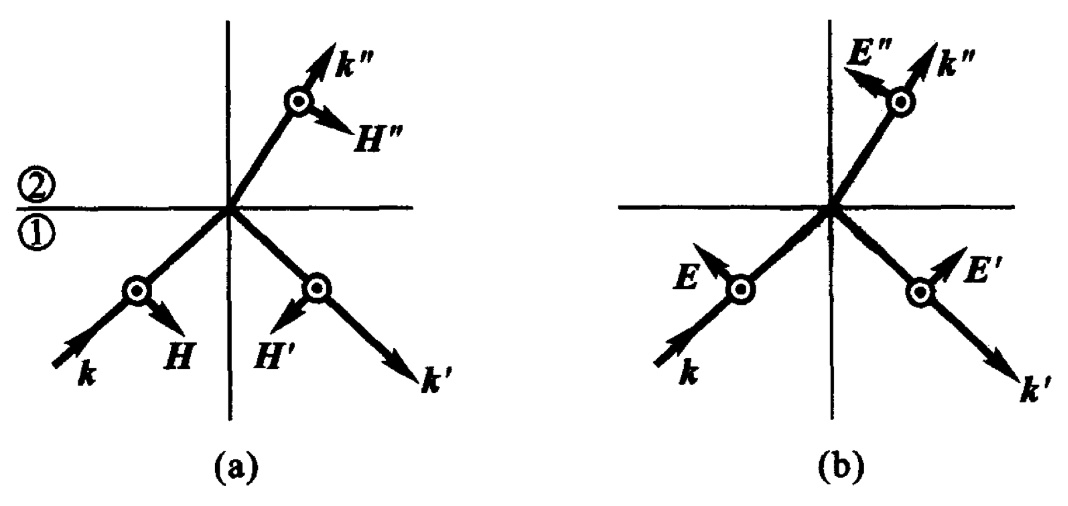
\includegraphics[width=0.8\linewidth]{figs/电场入射情况.jpg}
            \caption{电场入射方向} % 图片添加注释
            \end{figure}
        \begin{enumerate}[(1)]
            \item 电场垂直于入射面。直接根据边值关系写出
                    \begin{equation}
                        \begin{gathered}
                            E + E^{\prime} = E^{\prime\prime} \\
                            H \cos \theta - H^{\prime} \cos \theta^{\prime} =H^{\prime\prime} \cos \theta^{\prime\prime}
                        \end{gathered}
                    \end{equation}
                    
                    利用关系$H=\sqrt{\frac{\varepsilon}{\mu}}E$和$\mu= \mu_0$,并利用折射定律化简可以得到
                    \begin{equation}
                        \label{eq.4_32}
                        \boxed{\begin{aligned}
                        &\frac{E^{\prime}}{E}=\frac{\sqrt{\varepsilon_{1}} \cos \theta-\sqrt{\varepsilon_{2}} \cos \theta^{\prime \prime}}{\sqrt{\varepsilon_{1}} \cos \theta+\sqrt{\varepsilon_{2}} \cos \theta^{\prime \prime}}=-\frac{\sin \left(\theta-\theta^{\prime \prime}\right)}{\sin \left(\theta+\theta^{\prime \prime}\right)} \\
                        &\frac{E^{\prime \prime}}{E}=\frac{2 \sqrt{\varepsilon_{1}} \cos \theta}{\sqrt{\varepsilon_{1}} \cos \theta+\sqrt{\varepsilon_{2}} \cos \theta^{\prime \prime}}=\frac{2 \cos \theta \sin \theta^{\prime \prime}}{\sin \left(\theta+\theta^{\prime \prime}\right)}
                        \end{aligned}}
                    \end{equation}
            \item 电场平行于入射面。同理
            \begin{equation}
                \begin{gathered}
                    H + H^{\prime} = H^{\prime\prime} \\
                    E \cos \theta - E^{\prime} \cos \theta^{\prime} =E^{\prime\prime} \cos \theta^{\prime\prime}
                \end{gathered}
            \end{equation}

            同样代换电场和磁场可以得到
            \begin{equation}
                \label{eq.4_34}
                \boxed{\begin{gathered}
                \frac{E^{\prime}}{E}=\frac{\tan \left(\theta-\theta^{\prime \prime}\right)}{\tan \left(\theta+\theta^{\prime \prime}\right)} \\
                \frac{E^{\prime \prime}}{E}=\frac{2 \cos \theta \sin \theta^{\prime \prime}}{\sin \left(\theta+\theta^{\prime \prime}\right) \cos \left(\theta-\theta^{\prime \prime}\right)}
                \end{gathered}}
            \end{equation}
        \end{enumerate}
        \vspace*{2em}
        
        上式\ref{eq.4_32}和式\ref{eq.4_34}称为菲涅尔公式,阐述了入射波、反射波和折射波的强度关系。对于正常的电磁波,有各个方向偏振的成分,但是我们可以看到电场偏振方向的不同会有不同的反折射关系。恰好对于$\theta + \theta^{\prime}=90^\circ$的情况,根据式\ref{eq.4_34}可知,平行于边界面入射的电场反射波为零,即这时的反射波全部为垂直偏振的偏振光。\textbf{这是光学中的布儒斯特定律,满足$\theta + \theta^{\prime}=90^\circ$的角称为布儒斯特角}。

        菲涅尔公式也同样可以得出半波损失的结论——当$\varepsilon_2 > \varepsilon_1$时有$\theta > \theta^\prime$,则$E^\prime/E$为负数,反射波电场和入射波电场反相。

        我们经常用到反射系数R和投射系数T,分别代表光波强度的比值
        \begin{equation}
            \begin{gathered}
            R \equiv \frac{I_{\mathrm{R}}}{I_{1}}=\left(\frac{E_{0 \mathrm{R}}}{E_{01}}\right)^{2}=\left(\frac{n_{1}-n_{2}}{n_{1}+n_{2}}\right)^{2} \\
            T \equiv \frac{I_{\mathrm{T}}}{I_{1}}=\frac{\varepsilon_{2} v_{2}}{\varepsilon_{1} v_{1}}\left(\frac{E_{0 \mathrm{~T}}}{E_{01}}\right)^{2}=\frac{4 n_{1} n_{2}}{\left(n_{1}+n_{2}\right)^{2}}
            \end{gathered}
        \end{equation}

        \subsection{全反射关系}  
        由于全反射涉及到上节没有纳入考虑的一个新的波模,故另起一节做记录。由于折射角大于90$^\circ$之后就没有实数值能够表达了,我们需要另外寻找一个满足条件的波模。

        之前折射的关系仍然成立\[k^{\prime\prime}_x =k_x=k \sin \theta \]且根据振幅关系\[k^{\prime\prime}= k \frac{v_1}{v_2}=k n_{21}\]可以表达出z轴方向的波矢量分量,其已经表示为了一个虚数
        \begin{equation}
            k_{z}^{\prime \prime}=\sqrt{k^{\prime \prime 2}-k_{x}^{\prime \prime 2}}=\mathrm{i} k \sqrt{\sin ^{2} \theta-n_{21}^{2}}
        \end{equation}
        简记\[ \kappa=k \sqrt{\sin ^{2} \theta-n_{21}^{2}}\]则表示折射波电场
        \begin{equation}
            \boldsymbol{E}^{\prime \prime}=\boldsymbol{E}_{0}^{\prime \prime} \mathrm{e}^{-\kappa z} \mathrm{e}^{\mathrm{i}\left(k_{x}^{\prime \prime} x-\omega t\right)}
        \end{equation}
        注意这个波模在之前没有纳入考虑是因为在$z \to -\infty$的时候$ \boldsymbol{E^{\prime \prime} \to \infty}$,所以只出现在上半平面。相较于之前的波,它多了一个衰减项,该衰减层的厚度为
        \begin{equation}
            \kappa^{-1} = \frac{1}{k\sqrt{\sin ^2 \theta - n_{21}^2}}= \frac{\lambda_1}{2 \pi \sqrt{\sin ^2 \theta - n_{21}^2}}
        \end{equation}
        \begin{wrapfigure}{r}{6cm}%靠文字内容的右侧
            \centering
            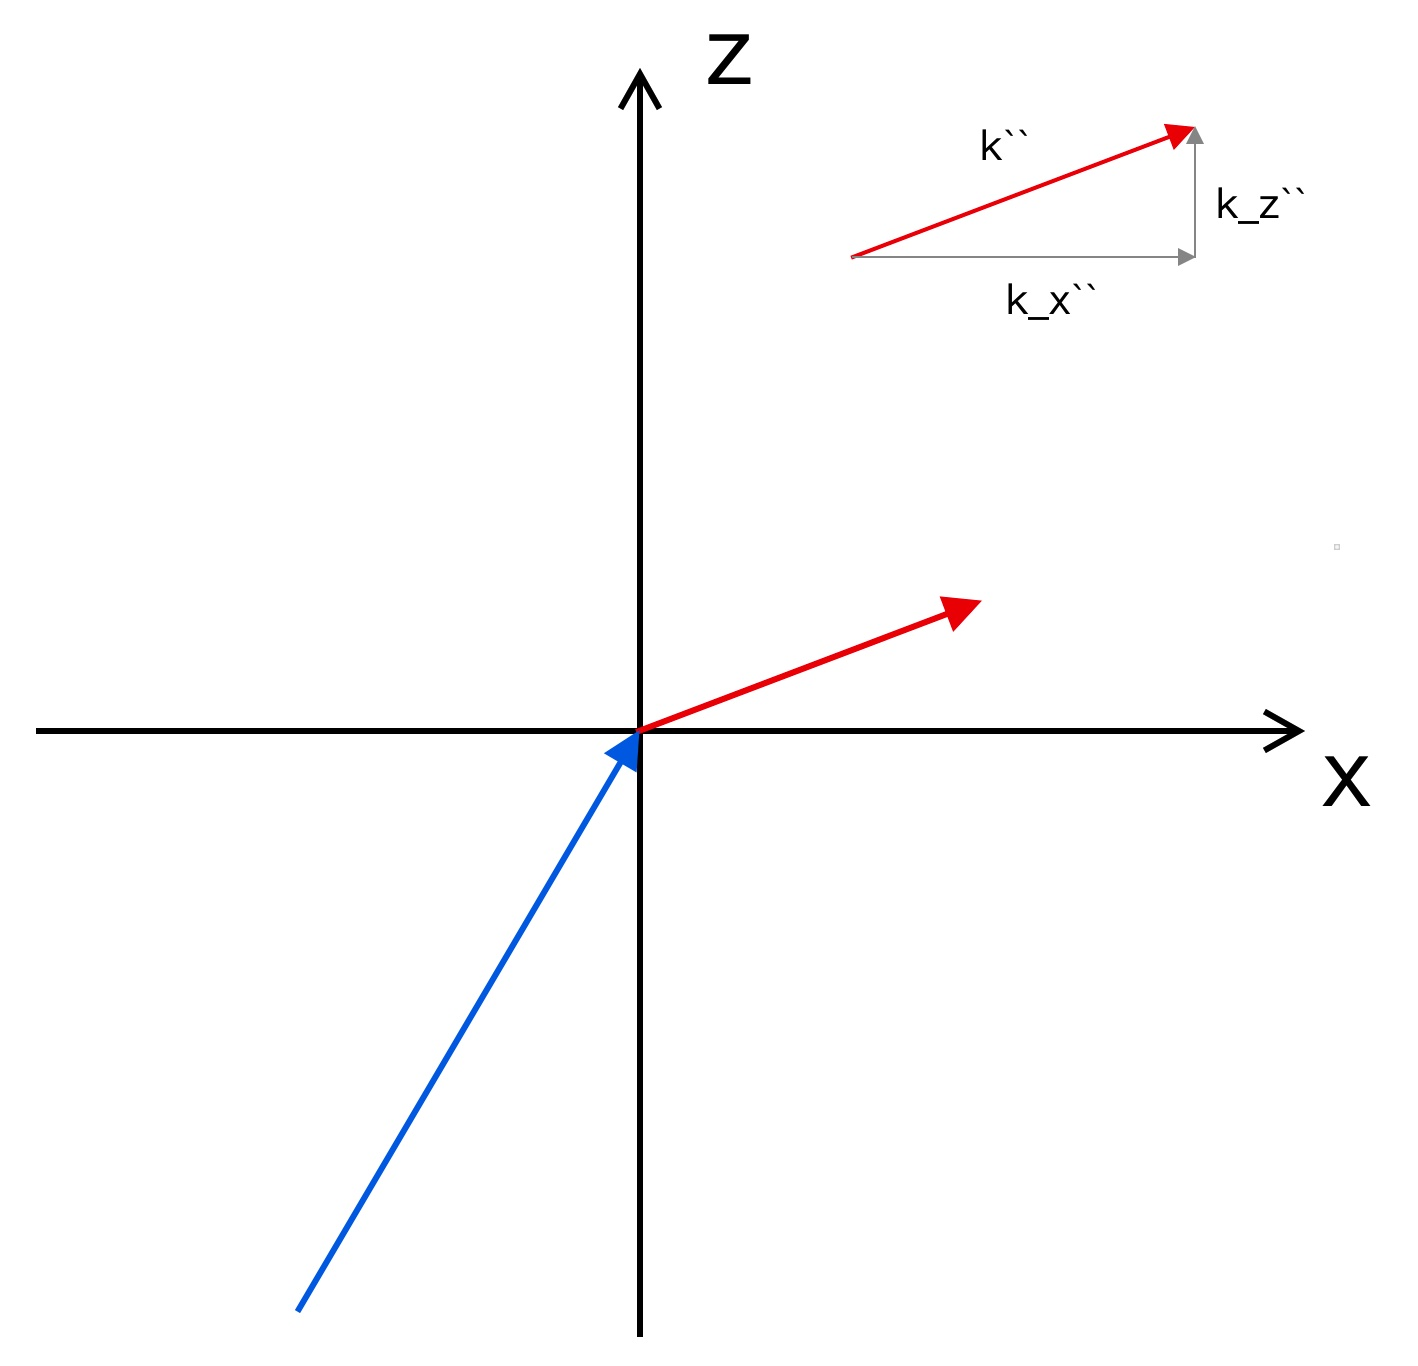
\includegraphics[width=0.34\textwidth]{figs/电磁场折射示意图.jpg}
            \caption*{\footnotesize 电磁场折射示意图}
            \end{wrapfigure}

        这种情况下菲涅尔公式依然适用,只是需要把$\sin \theta$的定义改变为
        \begin{equation}
            \begin{aligned}
            &\sin \theta^{\prime \prime} \rightarrow \frac{k_{x}^{\prime \prime}}{k^{\prime \prime}}=\frac{\sin \theta}{n_{21}} \\
            &\cos \theta^{\prime \prime} \rightarrow \frac{k_{z}^{\prime \prime}}{k^{\prime \prime}}=\mathrm{i} \sqrt{\frac{\sin ^{2} \theta}{n_{21}^{2}}-1}
            \end{aligned}
        \end{equation}
        就可以直接代入进行计算

        在全反射过程中,介质二是起到作用了的,在半个周期的时候,电磁能量透过第二介质并在界面的薄层储存起来,在另一个半周这些能量都释放出来变为反射能量。我们可以从折射层的能流密度看出,结合式\ref{eq.4_20}计算$\boldsymbol{H}$并由能流密度平均值公式\ref{eq.4_26}可以分别计算出x,z方向上的能流密度
        \begin{equation}
            \begin{aligned}
            &\bar{S}_{x}^{\prime \prime}=\frac{1}{2} \operatorname{Re}\left(E_{y}^{\prime \prime *} H_{z}^{\prime \prime}\right)=\frac{1}{2} \sqrt{\frac{\varepsilon_{2}}{\mu_{2}}} \mid E_{0}^{\prime \prime}{ }^{2} \mathrm{e}^{-2 kz} \frac{\sin \theta}{n_{21}} \\
            &\bar{S}_{z}^{\prime \prime}=-\frac{1}{2} \operatorname{Re}\left(E_{y}^{\prime \prime *} H_{x}^{\prime \prime}\right)=0
            \end{aligned}
        \end{equation}
        即进入介质层二的能流密度全都沿着x传播\footnote{\textcolor[RGB]{143,143,143}{Question:在z方向没有能流密度的话为什么该衰减层还有厚度呢?}}
\section{电磁波在导体内的传播}
    导体内的自由电子会收到电磁波的作用运动,反过来衰减电磁波的传播。在这个过程中,电磁能量不断转化为热量。
    \subsection{导体内的自由电荷的分布}
        我们首先来考虑导体中自由电荷运动满足的规律,我们可以知道电荷相对更聚集的地方就会自发的向周围流动,用数学语言表示为
        \begin{equation}
            \nabla \cdot \boldsymbol{J} = \sigma (\nabla \cdot \boldsymbol{E}) = \frac{\sigma}{\varepsilon}\rho
        \end{equation}
        由电荷守恒定律\[\frac{\partial \rho}{\partial t}=-\nabla \boldsymbol{J}=-\frac{\sigma}{\varepsilon}\rho\]可以解得
        \begin{equation}
            \rho(t) = \rho_0 e^{(-\frac{\sigma}{\varepsilon}t)}
        \end{equation}

        可以发现电荷密度随时间衰减,衰减的特征时间为
        \begin{equation}
            \tau =\frac{\varepsilon}{\sigma}
        \end{equation}

        如果入射电磁波的频率满足$\omega \ll \tau^{-1}$,电磁波就会在介质电荷变化不大的时候快速通过,可以认为这时候\[\rho(t)=0\]或者表示为
        \begin{equation}
            \frac{\sigma}{\varepsilon \omega} \ll 1
        \end{equation}
        我们称为\textbf{良导体条件}。如果电磁波的频率不太高,一般金属导体都可以视作良导体,良导体内部没有净的自由电荷积聚,电荷都分布在导体表面上。
    \subsection{导体内的电磁波}
        相较于介质中的电磁波,我们只需要加入一个电流引起的变化项,直接给出对于一定频率的电磁波在导体内的麦克斯韦方程
        \begin{equation}
            \begin{gathered}
            \boldsymbol{\nabla} \times \boldsymbol{E}=\mathrm{i} \omega \mu \boldsymbol{H} \\
            \boldsymbol{\nabla} \times \boldsymbol{H}=-\mathrm{i} \omega \varepsilon\boldsymbol{E}+\sigma \boldsymbol{E} \\
            \boldsymbol{\nabla} \cdot \boldsymbol{E}=0 \\
            \boldsymbol{\nabla} \cdot \boldsymbol{H}=0
            \end{gathered}
        \end{equation}
        我们也可以直接把由导体电荷分布引起的这一项和之前的介电常数合并写作“复电容率”,记为
        \begin{equation}
            \varepsilon^\prime = \varepsilon + i \frac{\sigma}{\omega}
        \end{equation}
        则麦氏方程的第二项写作\[\boldsymbol{\nabla} \times \boldsymbol{H}=-\mathrm{i} \omega \varepsilon^\prime \boldsymbol{E}\]方程其他项完全一致,只需要将介质中的解的$\varepsilon$项改为复电容率就可以得到介质中的解。 

        简单介绍一下复电容率各项的物理意义,其实数项代表位移电流的作用,不消耗电场的功率;复数项为传导电流的作用,会引起能量耗散\footnote{其实对于介质而言,我们将电磁场在介质中耗散的情况,介质的电容率也是一个复数}。

        引入复电容率后我们就可以直接写出Helmholtz公式
        \begin{equation}
            \begin{gathered}
                \nabla^2 \boldsymbol{E} + k^2 \boldsymbol{E} = 0 \\
                k = \omega \sqrt{\mu \varepsilon^\prime}
            \end{gathered}
        \end{equation}
        为进一步考虑k变为复数对整个电磁波解的影响,我们将k写作实部和虚部的分量形式\footnote{其实可能你已经发现了,在上一节讨论全反射关系的时候就已经考虑到k为复数的情况了——这会给电磁波解带来一个衰减项}
        \begin{equation}
            k = \boldsymbol{\beta}+ i \boldsymbol{\alpha}
        \end{equation}
        则还是考虑最简单的平面电磁波的情况,其电磁波可以表示为
        \begin{equation}
            \label{eq.4_49}
            \boldsymbol{E} = \boldsymbol{E_0}e^{i \boldsymbol{k}\cdot x} = \boldsymbol{E_0} e^{- \boldsymbol{\alpha} \cdot x} e^{i(\boldsymbol{\beta} \cdot x - \omega t)}
        \end{equation}
        很明显,虚部$\boldsymbol{\alpha}$是一个衰减常数。

        我们希望能够用具体的物理量表示出$\alpha$和$\beta$。代入复电容率的关系得到\[k^{2}=\beta^{2}-\alpha^{2}+2 \mathrm{i} \boldsymbol{\alpha} \cdot \boldsymbol{\beta}=\omega^{2} \mu\left(\varepsilon+\mathrm{i} \frac{\sigma}{\omega}\right)\]比较实部和虚部就可以得到
        \begin{equation}
            \label{eq.4_50}
            \begin{gathered}
                \beta^2 - \alpha^2 = \omega^2 \mu \varepsilon \\
                \boldsymbol{\alpha} \cdot \boldsymbol{\beta}= \frac{1}{2}\omega \mu \sigma
            \end{gathered}
        \end{equation}
        由于$\boldsymbol{\alpha}$和$\boldsymbol{\beta}$的方向还不确定,只靠上式还不能具体给出其表达式,需结合边界条件给出\footnote{郭硕鸿先生的教材中举了一个简单的例子,有兴趣可自行翻阅}。
    \subsection{趋肤效应和穿透深度}
        我们简述一下电磁波在导体内传播的规律:电磁波一般只在介质中和导体之外的地方传播。在导体界面上,电磁波和导体的自由电荷作用形成传导电流,电流的存在使电磁波向外反射,一部分电磁能量透入导体内,随传导电流的作用逐渐转换为焦耳热。

        我们考虑最简单的垂直入射的情况,因为这样就只需要考虑z方向的分量。可以将式\ref{eq.4_49}写为\[\boldsymbol{E} =\boldsymbol{E_0} e^{- \alpha z} e^{i(\beta z - \omega t)}\]确定$\alpha$和$\beta$的方向之后就可以根据式\ref{eq.4_50}可以解出$\alpha$和$\beta$:
        \begin{equation}
            \begin{aligned}
            &\beta=\omega \sqrt{\mu \varepsilon}\left[\frac{1}{2}\left(\sqrt{1+\frac{\sigma^{2}}{\varepsilon^{2} \omega^{2}}}+1\right)\right]^{\frac{1}{2}} \\
            &\alpha=\omega \sqrt{\mu \varepsilon}\left[\frac{1}{2}\left(\sqrt{1+\frac{\sigma^{2}}{\varepsilon^{2} \omega^{2}}}-1\right)\right]^{\frac{1}{2}}
            \end{aligned}
            \end{equation}
        这个式子还是显得有些繁琐,对于良导体的情形,$k^2$的实部可以忽略,有近似关系式
        \begin{equation}
            \begin{gathered}
            k^{2} \approx \mathrm{i} \omega \mu \sigma \\
            k \approx \sqrt{\mathrm{i} \omega \mu \sigma} \approx \beta+\mathrm{i} \alpha
            \end{gathered}
        \end{equation}
        可以得到\footnote{为方便记忆你可以认为由\ref{eq.4_50}直接拆开得到}
        \begin{equation}
            \alpha \approx \beta \approx \sqrt{\frac{\omega \mu \sigma}{2}}
        \end{equation}

        还记得我们最开始的目的就是试图表达电磁波在导体的穿透深度。我们\textbf{将波幅降至导体表面原值的$1/e$时的传播距离称为穿透深度$\sigma$},很显然就是$\alpha$的平方
        \begin{equation}
            \boxed{\delta = \frac{1}{\alpha} = \sqrt{\frac{2}{\omega \mu \sigma}}}
        \end{equation}
        可以看到穿透深度的平方和电导率以及电磁波的频率成反比。我们想要知道电场和磁场谁在导体中的传播更加重要,同样给出两者的比值
        \begin{equation}
            \label{eq.4_55}
            \begin{gathered}
                \boldsymbol{H}=\frac{1}{\omega \mu} \boldsymbol{k} \times \boldsymbol{E}=\frac{1}{\omega \mu}(\beta+\mathrm{i} \alpha) \boldsymbol{e}_{\mathrm{n}} \times \boldsymbol{E} \\
                \boldsymbol{H} \approx \sqrt{\frac{\sigma}{\omega \mu}} \mathrm{e}^{\mathrm{i} \frac{\mathrm{\pi}}{4}} \boldsymbol{e}_{\mathrm{n}} \times \boldsymbol{E} \\
                \sqrt{\frac{\mu}{\varepsilon}}\left|\frac{\boldsymbol{H}}{\boldsymbol{E}}\right|=\sqrt{\frac{\sigma}{\omega \varepsilon}} \gg>1
            \end{gathered}
        \end{equation}
        可以看到在良导体中,电磁波的能量主要是磁场能量\footnote{\textcolor[RGB]{143,143,143}{Question:在一般单位制下可以直接理解为磁场要比电场强吗,这样的话由式\ref{eq.4_21}可以说在真空中电磁场的主要能量是电场能量?}}
    \subsection{在导体表面的反射}
        只考虑垂直入射的情况,我们有关系\[E - E^\prime = E^{\prime \prime}, \quad H- H^\prime=H^{\prime \prime}\]分别结果真空和介质中磁场的关系可以(参见式\ref{eq.4_20}和\ref{eq.4_55})转化为电场写出第二式\[E-E^{\prime}=\sqrt{\frac{\sigma}{2 \omega \varepsilon_{0}}}(1+\mathrm{i}) E^{\prime \prime}\]就可以连立写出电场的比值为
        \begin{equation}
            \frac{E^\prime}{E} = -\frac{1+i-\sqrt{\frac{2 \omega \varepsilon_0}{\sigma}}}{1+i+\sqrt{\frac{2 \omega \varepsilon_0}{\sigma}}}
        \end{equation}
        更常用的是反射系数
        \begin{equation}
            R=\left|\frac{E^{\prime}}{E}\right|^{2}=\frac{\left(1-\sqrt{\frac{2 \omega \varepsilon_{0}}{\sigma}}\right)^{2}+1}{\left(1+\sqrt{\frac{2 \omega \varepsilon_{0}}{\sigma}}\right)^{2}+1} \approx 1-2 \sqrt{\frac{2 \omega \varepsilon_{0}}{\sigma}}
        \end{equation}

        从上式可以看出,电导率越高越容易反射,波长越长的电磁波越容易被反射。